\documentclass[a4paper,10pt]{article} % Default font size and paper size

\usepackage{style}

\begin{document}

\pagestyle{empty} % Removes page numbering

%----------------------------------------------------------------------------------------
%	NAME AND CONTACT INFORMATION
%----------------------------------------------------------------------------------------

\par{\centering{\Huge Alexey \textsc{Ryabykin}}\bigskip\par} % Your name

\section{Personal Data}

    \begin{tabular}{rl}
    \begin{tabular}{rl}
        \textsc{Date of Birth:} & 11 September 2000 \\
        \textsc{Address:} & Solntsevsky Avenue, 7k1, Moscow, Russia \\
        \textsc{Phone:} & +7 (999) 608-92-52\\
        \textsc{email:} & \href{mailto:ryabykin.as@yandex.ru}{ryabykin.as@yandex.ru}\\
        \textsc{Github:} & \href{https://github.com/addicted-by}{https://github.com/addicted-by}
        \end{tabular} \hspace*{1cm}
        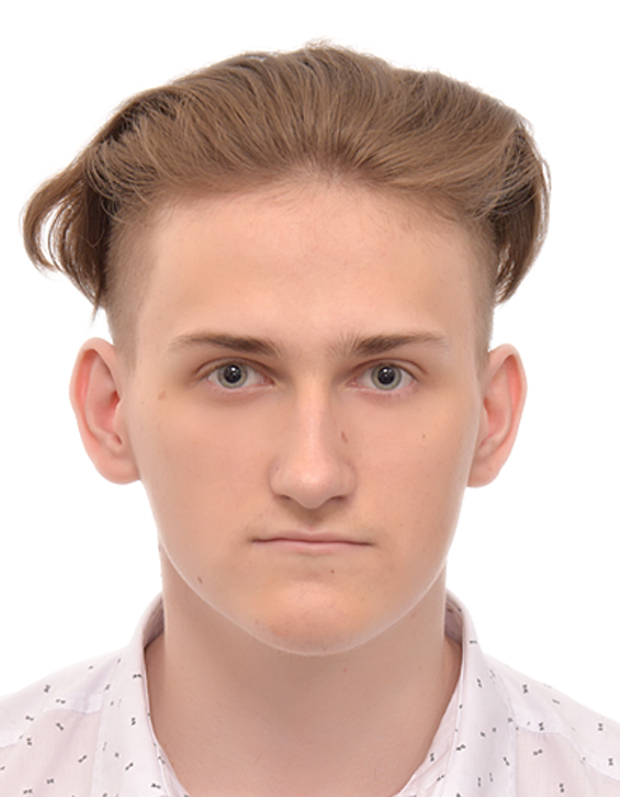
\includegraphics[scale=0.7, valign=c]{cv.jpg}
    \end{tabular}

%----------------------------------------------------------------------------------------
%	EDUCATION
%----------------------------------------------------------------------------------------

\section{Education}
\begin{tabular}{cp{10.5cm}}	
\textsc{August} 2022 -- \textsc{Today} & Master of Applied Mathematics and Informatics, Data Science, \textbf{Higher School of Economics}, Moscow\\
\\
\textsc{July} 2022 & Bachelor of Applied Mathematics, \textbf{Moscow Aviation Institute}, Moscow\\
& Thesis: ``Quantifying Public Opinion and Consumer Preferences by \\&Semantic Analysis Methods Algorithm.'' | \small Advisor: Prof. Egor \textsc{Sukhov}\\
&\normalsize \textsc{Gpa}: 4.67/5.0\hyperlink{grds}{\hfill | \footnotesize Detailed List of Exams}\\
&\\
\end{tabular}


% ----------------------------------------------------------------------------------------
% 	COMPUTER SKILLS 
% ----------------------------------------------------------------------------------------


\section{Computer Skills}

\begin{tabular}{p{13cm}}
    \textsc{Intermediate Knowledge:} \vspace*{3.33pt}

    \begin{center}
    \begin{itemize}
        \item[] \py{\small{\textsc{pandas}}} \py{\textsc{torchtext}} \py{\textsc{torchvision}} \py{\textsc{keras}} \py{\textsc{pytorch}} \py{\textsc{scikit-learn}}\\[3.33pt]  \mytcbox{\textsc{NLP}} \mytcbox{\textsc{CV}} \py{\textsc{tensorflow}} \mytcbox{\textsc{Data Visualization}} \mytcbox{\textsc{Data Mining}} \mytcbox{\sffamily\LaTeX}  \setmainfont[SmallCapsFont=Fontin-SmallCaps.otf]{Fontin-Regular.otf}
\end{itemize}
\end{center}
\vspace*{8pt}

\textsc{Basic Knowledge:} \vspace*{3.33pt}

\begin{center}
    \begin{itemize}
        \item[] \mytcbox{\textsc{C++}} \mytcbox{\textsc{html}} \mytcbox{\textsc{MLOps}} \mytcbox{\textsc{SQL}} \py{\textsc{xgboost}} \py{\textsc{optuna}} \mytcbox{\textsc{Docker}} \mytcbox{\textsc{Linux}} \mytcbox{\textsc{git}} \py{\textsc{Flask}} \\[3.33pt] \mytcbox{\textsc{CSS}} \mytcbox{\textsc{Unity}} \py{\textsc{Selenium}} \mytcbox{\textsc{Google Cloud AI Platform}}
    \end{itemize}
    \end{center}
\end{tabular}

\section{Publications}
\begin{tabular}{r|p{11cm}}
    \textsc{Article} & Ryabykin A., Sukhov. E. 
    Neural methods in the sentiment analysis task.
    ``DSPA: digital signal processing application surveys (No2-2022)''. P. 41. 2022. \href{http://media-publisher.ru/wp-content/uploads/DSPA-2-2022.pdf}{\hfill | \footnotesize{Paper}}\\ \multicolumn{2}{c}{}\\
    \textsc{Thesis} & Ryabykin A., Sukhov. E.
     The real-time weapon detection by neural networks for security and intelligence services. 
     ``Gagarin Reading 2022''. P. 464. 2022. \href{https://drive.google.com/file/d/1E3AIVA1ELlAft27UQeW1dJcybUhdjCsJ/view?usp=sharing}{\hfill | \footnotesize Paper}\\
    
\end{tabular}

\section{Training}
\begin{tabular}{rp{9cm}}
    \textsc{February-July} 2022 & Deep Learning School\\

    \textsc{May} 2022 & School of Mathematical Modeling \footnotesize(winner in predictive analytics in aviation task)\normalsize\\

    \textsc{March-April} 2022 & RuCode Festival 5.0 \footnotesize(additional education and top25\%)\normalsize

    \end{tabular}

\section{Projects}
\begin{tabular}{p{13cm}}
\begin{center}\vspace*{-7.8pt}

\begin{enumerate}[wide, itemsep=6.66pt, leftmargin=*]
    \item \textsc{Style transfer telegram bot} \href{https://github.com/addicted-by/nst_bot}{\hfill | \footnotesize Link}\\[3.33pt] Asynchronized telegram with simple database to neural photo stylization\\[3.33pt] \textsc{Stack}: \py{aiogram} \py{sqlite} \py{torch} \py{torchvision} \mytcbox{GAN}
    \item \textsc{Sentiment analysis web application} \href{https://github.com/addicted-by/widget}{\hfill | \footnotesize Link}\\[3.33pt] Implementation of the ensembled neural classification models and \textsc{BERTopic} to the web site \\[3.33pt] \textsc{Stack}: \py{Flask} \html{\textsc{Bootstrap}} \py{huggingface} \py{torchtext} \mytcbox{\textsc{Topic Modeling}}
    \item \textsc{Real-Time weapon detection telegram bot} \href{https://github.com/addicted-by/CV/tree/main/weapon_detector_bot}{\hfill | \footnotesize Link}\\[3.33pt] Asynchronized telegram with simple database to neural photo stylization\\[3.33pt] \textsc{Stack}: \py{TelegramBotAPI} \py{torch} \py{\textsc{opencv}} \mytcbox{\textsc{Transfer Learning}}
    \item \textsc{Predictive analysis} \href{https://github.com/addicted-by/predictive_analysis}{\hfill | \footnotesize Link}\\[3.33pt] Synthetic data generation to increase the quality of failure predictions in a mechanical systems \\[3.33pt] \textsc{Stack}: \py{torch} \mytcbox{\textsc{Time Series}} \mytcbox{\textsc{Anomaly Detection}} \py{pyfmi} \mytcbox{\textsc{OpenModelica}}
\end{enumerate} \vspace*{-10pt}
\end{center}
\end{tabular}
    
\section{Achievments}
\begin{tabular}{rp{8cm}r}
    \textsc{March} 2022 & Changellenge\>\> CUP IT 2022 Data Science \footnotesize(high quality award)\normalsize&\href{https://drive.google.com/file/d/1nzJZvqc1fVry3vje4rqn_khu6yu5ZKk9/view?usp=sharing}{\hfill | \footnotesize Certificate}\\

    \textsc{March-May} 2021 & CROC\>\> Case Laboratory \footnotesize(task distribution case)\normalsize&\href{https://drive.google.com/file/d/1pMN4490Kn86PVl2UGvcGSIRORIqeMZGi/view?usp=sharing}{\hfill | \footnotesize Certificate}
    \end{tabular}
% CROC case laboratory
% High Quality Award
% ISS HACK
%----------------------------------------------------------------------------------------
%	LANGUAGES
%----------------------------------------------------------------------------------------

\section{Languages}

\begin{tabular}{rl}
\textsc{English:} & Fluent\\

\textsc{Russian:} & Mothertongue\\

\end{tabular}

\section{Relevant Courses}
\begin{tabular}{rp{11cm}r}
    \textsc{August 2021} & Basics of C++ development: Yellow Belt \footnotesize(99.93\%)\normalsize\href{https://coursera.org/share/bd93be1044642b0f76be5859fbf1b96f}{\hfill | \footnotesize Certificate}\\
    \textsc{July 2021} &  Basics of C++ development: White Belt \footnotesize(100\%)\normalsize\href{https://coursera.org/share/f696a9c66143059a301f9f1e5d2bcca8}{\hfill | \footnotesize Certificate}\\
    \textsc{July 2021} &  Machine Learning: Language Processing \footnotesize(100\%)\normalsize\href{https://coursera.org/share/f91409b5a5184193be1017168afb7952}{\hfill | \footnotesize Certificate}\\
    \textsc{May 2021} & Supervised Learning \footnotesize(96.75\%)\normalsize\href{https://coursera.org/share/c877829114f8b67d7cc8a44057f4e571}{\hfill | \footnotesize Certificate}\\
    \textsc{November 2021} & Data Introduction \footnotesize(93.16\%)\normalsize\href{https://coursera.org/share/bd93be1044642b0f76be5859fbf1b96f}{\hfill | \footnotesize Certificate}\\
    \textsc{November 2021} & Math and Python for Data Science \footnotesize(100\%)\normalsize\href{https://coursera.org/share/b5ca152259931c53eb6cc4fff4203582}{\hfill | \footnotesize Certificate}\\
    \textsc{October 2021} & SQL for Data Science \footnotesize(92.06\%)\normalsize\href{https://coursera.org/share/8cf7fb85c6eed6291d92f67fcede0d92}{\hfill | \footnotesize Certificate}
\end{tabular}


%----------------------------------------------------------------------------------------
%	INTERESTS AND ACTIVITIES
%----------------------------------------------------------------------------------------

\section{Interests and Activities}

Programming, Open-Source, ML\\
Genetics, Psychoanalysis, Neurobiology\\
Gym, Running

%----------------------------------------------------------------------------------------

\newpage

%----------------------------------------------------------------------------------------
%	GRADE TABLES
%----------------------------------------------------------------------------------------

\par{\centering\Large \hypertarget{grds}{Bachelor of Applied Mathematics}\par}\large{\centering Grades\par}\normalsize

\begin{center}
\begin{tabular}{lcc}
\multicolumn{1}{c}{\textsc{Exam}} & \textsc{Grade}&\textsc{Credit Hrs}\\ \hline
DataBases & 5 & 5\\
Linear Algebra and Analytic Geometry & 5 & 7\\
Mathematical Analysis & 5 & 16\\
Mathematical Logic & 4 & 8\\
Differential Equations & 5 & 5\\
Physics	& 4 & 8\\	
Probability Theory and Mathematical Statistics & 4 & 7\\
Optimization Methods & 5 & 4\\
Numerical Methods & 5 & 6\\
Theoretical mechanincs & 4 & 6\\
Computer Math & 4 & 4\\
History & 5 &	4\\ \\

Mathematical Methods in Economics & 4 & 4\\
Machine Learning with Python & 5 & 5\\
Control Theory & 5 & 4\\
Object-Oriented Modeling of Dynamic Processes & 5 & 5\\
Random Processes & 4 & 4\\
Functional Analysis	 & 4 & 6\\ \\

Educational Practices & 5 & 15\\		
Final Thesis & 5 & 9\\	
& Total & 132\\\cline{2-3}
&\textsc{Gpa}&\textbf{4.67/5.0}
\end{tabular}
\end{center}
\end{document}
